%%
%% This is file `sample-sigchi.tex',
%% generated with the docstrip utility.
%%
%% The original source files were:
%%
%% samples.dtx  (with options: `sigchi')
%% 
%% IMPORTANT NOTICE:
%% 
%% For the copyright see the source file.
%% 
%% Any modified versions of this file must be renamed
%% with new filenames distinct from sample-sigchi.tex.
%% 
%% For distribution of the original source see the terms
%% for copying and modification in the file samples.dtx.
%% 
%% This generated file may be distributed as long as the
%% original source files, as listed above, are part of the
%% same distribution. (The sources need not necessarily be
%% in the same archive or directory.)
%%
%% The first command in your LaTeX source must be the \documentclass command.
\documentclass[sigchi]{acmart}

%%
%% \BibTeX command to typeset BibTeX logo in the docs
% \AtBeginDocument{%
%   \providecommand\BibTeX{{%
%     \normalfont B\kern-0.5em{\scshape i\kern-0.25em b}\kern-0.8em\TeX}}}
\AtBeginDocument{%
  \providecommand\BibTeX{{%
    \normalfont B\kern-0.5em{\scshape i\kern-0.25em b}\kern-0.8em\TeX}}}

\settopmatter{printacmref=false} % Removes citation information below abstract
\renewcommand\footnotetextcopyrightpermission[1]{} % removes footnote with conference information in first column
\pagestyle{plain} % removes running headers
\usepackage{caption}
\usepackage{svg}
\usepackage{graphics}
\usepackage{amsmath}
\usepackage[british]{babel}
\usepackage{xcolor}
\usepackage{CJKutf8}
% \usepackage{cite}
% \usepackage{graphicx}
\usepackage{subcaption}
\usepackage{listings}
\usepackage{color}
% \usepackage{graphicx}
\usepackage{subcaption}
\definecolor{dkgreen}{rgb}{0,0.6,0}
\definecolor{gray}{rgb}{0.5,0.5,0.5}
\definecolor{mauve}{rgb}{0.58,0,0.82}

\lstset{frame=tb,
  language=C,
  aboveskip=3mm,
  belowskip=3mm,
  showstringspaces=false,
  columns=flexible,
  basicstyle={\small\ttfamily},
  numbers=none,
  numberstyle=\tiny\color{gray},
  keywordstyle=\color{blue},
  commentstyle=\color{dkgreen},
  stringstyle=\color{mauve},
  breaklines=true,
  breakatwhitespace=true,
  tabsize=3
}
%% Rights management information.  This information is sent to you
%% when you complete the rights form.  These commands have SAMPLE
%% values in them; it is your responsibility as an author to replace
%% the commands and values with those provided to you when you
%% complete the rights form.
% \setcopyright{}
% \copyrightyear{}
% \acmYear{}
% \acmDOI{}

%% These commands are for a PROCEEDINGS abstract or paper.
% \acmConference[Woodstock '18]{Woodstock '18: ACM Symposium on Neural
%   Gaze Detection}{June 03--05, 2018}{Woodstock, NY}
% \acmBooktitle{Woodstock '18: ACM Symposium on Neural Gaze Detection,
%   June 03--05, 2018, Woodstock, NY}
% \acmPrice{15.00}
% \acmISBN{978-1-4503-9999-9/18/06}


%%
%% Submission ID.
%% Use this when submitting an article to a sponsored event. You'll
%% receive a unique submission ID from the organizers
%% of the event, and this ID should be used as the parameter to this command.
%%\acmSubmissionID{123-A56-BU3}

%%
%% The majority of ACM publications use numbered citations and
%% references.  The command \citestyle{authoryear} switches to the
%% "author year" style.
%%
%% If you are preparing content for an event
%% sponsored by ACM SIGGRAPH, you must use the "author year" style of
%% citations and references.
%% Uncommenting
%% the next command will enable that style.
%%\citestyle{acmauthoryear}

%%
%% end of the preamble, start of the body of the document source.
\begin{document}

%%
%% The "title" command has an optional parameter,
%% allowing the author to define a "short title" to be used in page headers.
\title{Literature study \\
       Increasing resource utilization of cloud }

%%
%% The "author" command and its associated commands are used to define
%% the authors and their affiliations.
%% Of note is the shared affiliation of the first two authors, and the
%% "authornote" and "authornotemark" commands
%% used to denote shared contribution to the research.
\author{You Hu}
\email{adolphus.hu@student.vu.nl}
\affiliation{%
  \institution{VU Amsterdam }
%   \city{Amsterdam}
}



%%
%% By default, the full list of authors will be used in the page
%% headers. Often, this list is too long, and will overlap
%% other information printed in the page headers. This command allows
%% the author to define a more concise list
%% of authors' names for this purpose.
\renewcommand{\shortauthors}{You Hu}

%%
%% The abstract is a short summary of the work to be presented in the
%% article.



%%
%% Keywords. The author(s) should pick words that accurately describe
%% the work being presented. Separate the keywords with commas.


%%
%% This command processes the author and affiliation and title
%% information and builds the first part of the formatted document.
\maketitle

\section{Introduction}
The Netherlands eScience Center has developed solutions for calibrating imaged observation collected by LOw Frequency Array(LOFAR) telescope\footnote{\url{http://www.lofar.org/}}.
The LOFAR consists of 51 stations cross Europe and a typical LOFAR observation has the size of 100TB, after frequency averaging, the size can be reduced to 16TB. \cite{Spreeuw2019}
Collectively, there are over 5 PB of data will be stored each year. \cite{Start2020} 
This large volume of data requires vast computation availability to calibrate, on the other hand, since the process availability is not able to catch up with the data producetion, the observation will be processed when it is needed.

The current solutions , MPI, and Spark, will lead to a waste of computation resources in non-dedicated clusters. It can be visualized as Fig. \ref{fig:waste_cluster}.
\begin{figure}[h!]
  \begin{subfigure}[b]{0.45\textwidth}
      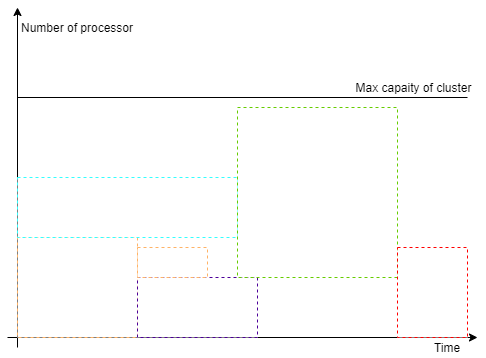
\includegraphics[width=\textwidth]{img/MPI_batch.png}
      \caption{Resources utilization of MPI batch jobs on cluster}
      \label{fig:MPI_batch}
  \end{subfigure}
  \begin{subfigure}[b]{0.45\textwidth}
      
\includegraphics[width=\textwidth]{img/spark_NP.png}
      \caption{Resources utilization of Spark on cluster}
      \label{fig:spark_np}
  \end{subfigure}
  \caption{The waste of compuation on cluster}\label{fig:waste_cluster}
\end{figure}
As it is shown in Fig. \ref{fig:MPI_batch}, MPI jobs are scheduled as fixed batch jobs which are colored boxes in the figure. It is very common to meet the situation that all jobs in the queue are too large and the number of idle resources is not enough for the jobs in the queue. 
For the Spark version, the possible situation can be visualized as Fig. \ref{sub@fig:spark_np}. The nodes should be reserved for Spark in advance and Spark task manager handles the task scheduling. For typical Spark applications relying on RDD, the number of required executors can be up and down dynamically. Part of computation resources may be wasted since this computation power is exclusive for Spark.
However, of course, the current Spark implementation for calibration is based on Driver mode and the granularity is one executor per task. In this case, the waste of resources won't happen within the Spark cluster. But when there are a lot of idle nodes in the cluster that not reserved for Spark at the beginning, they can not be used for Spark. 

In this project, we try to tackle on the issue of resource utilization. The LOFAR owns computation facility their own. Therefore, we take both perspectives of  cloud provider in Section 2 and cloud user in Section 3 into discussion.

\section{Cloud provider perspective}
The cloud providers own data centers with large quantity of and kinds of facilities. 
The resource management is the key point that the cloud provider will concern.
In 2013, Jennings and Stadler made a survey and listed challenges on Cloud resource management \cite{Jennings2015}.
They firstly lists actors in the cloud economy and then the fields of cloud technologies. 
Manvi and Shyam also made a survey on the same topic but it mainly focuses on IaaS cloud related aspects \cite{Manvi2014}. 
As it provides more observation from the technology side, the issues and definition of resource in clouds are given firstly.
In this section, the metrics around cloud are listed, as they are usually as the counterpart of resource utilization for trade off making.
And then, few related topics in the resource management field will be discussed.

\subsection{Metrics related to resource utilization}
In the cloud environment, there are many kinds of resources and a set of aspects around the cloud economy.
Both Jennings \cite{Jennings2015} and Manvi \cite{Manvi2014} starts with the definition of resources.

Jennings et al. categorize the resources into: compute, networking, storage, and power. 
Manvi at al. summarizes that there are physical resources(CPU,memory, storage, network elements and sensors ) and logical resources(OS, engergy, Network throughput/bandwidth,Load balancing mechanisms and so on).
There are overlap between two of them especially in the physical part, while Manvi adds API, OS, load balancing to logical resource concept.
However, it is understandable that API , OS and some protocols and mechanisms  can be viewed as some sort of asset of cloud owner, but they are more acceptable to be considered as part of Quality of Service(QoS) which needs resources to fulfill.
Therefore, in this section, we mainly focus on the utilization of physical resources like CPU, memory, storage; and consider the trade-off between utilization rate and QoS.

QoS (Quality of Service) metrics are import to both cloud provider and consumer, they are good for optimizing resource utilization efficiency
Bardsiri and Hashemi listed detailed metrics from four kinds of features:performance, economic, security and general. \cite{Bardsiri2014}
Their coverage is comprehensive. There are plenty of features and corresponding metrics that cloud users would put concern.

Given the background of researching utilization under limited resources, there are few metrics we consider important. 
For performance features, the CPU load rate and packet loss frequency are what users may concern while the cloud provides needs to make a compromise for utilization of resources.
In the economic aspect, the price per resource unit is the key point that cloud  providers and users wrestle on. However, from the technical view, the time for VM booting/deleting/suspending/provison attract more attantion.
Besides, the availability and reliability are very important. The response time is the key metric for auto-scaling mechanism.
Cloud providers need to pay effort on fault tolerance to make sure the safety of the cloud.

In the following sections, we will explore how cloud providers face resource management issues and the metrics shown above play important roles in  those researches.

\subsection{Resource demand profiling }
There is no doubt that before allocation and provision, it is vital to estimate the demanded resource of each workload. In this section, the workloads can be classified as two types: batch and interactive.
Different workload has different nature of their requirement of resources. 

For the batch applications, it is easier to estimate the resource demand. Given the parameters of each pre-identified application, the required resource over time can be calculated by a pre-trained model.
As an example, Becerra et al. purposed a methodology to profile the batch jobs. \cite{becerra2009batch} 
The workload profile is updated according  to the deviation  of CPU, memory, network usage by the time. 
% Besides of this typical approach, in Spark ecosystem, the resource demand can be calculated much more easier as each Spark batch job can be parsed to Directed Acyclic Graph(DAG) and the demanded resource in each state can be estimated.
% According to this feature, Databrick implements  auto-scaling mechanism\footnote{\url{https://databricks.com/blog/2018/05/02/introducing-databricks-optimized-auto-scaling.html}} within it the required resources can be dynamically calculated.

It is clear that the workload of web applications varies dynamically over multiple time scales. One approach is that all the workloads are 

\newpage  
\bibliography{sample-base.bib}
\bibliographystyle{ACM-Reference-Format}

\end{document}
\endinput
%%
%% End of file `sample-sigchi.tex'.

